
\chapter{Introducción}\label{cap:cap1}

En el competitivo y dinámico mundo del comercio minorista, la gestión eficiente de un negocio especializado es crucial para su éxito y sostenibilidad. Este Trabajo Final de Máster se enfoca en los desafíos específicos de un negocio dedicado a la venta de artículos de pesca, un nicho que requiere soluciones innovadoras para la gestión del inventario, la facilitación de ventas en línea y la posibilidad para el cliente de reservar cebo con antelación. 

\vspace{0.5cm}

El objetivo principal de este proyecto es el desarrollo de una aplicación web integral que aborde las necesidades específicas de un negocio de artículos de pesca. Para ello, se emplearán tecnologías de vanguardia como Laravel en el Back-end y Angular en el Front-end, asegurando una plataforma robusta y eficiente. La aplicación permitirá gestionar de manera efectiva el inventario de productos, ofreciendo a los clientes la posibilidad de realizar compras en línea y resevar cebo y a los administradores del negocio la capacidad de gestionar la plataforma web, los productos y las reservas de cebo.

\vspace{0.5cm}

Además de las funcionalidades mencionadas, se busca garantizar una experiencia de usuario intuitiva y fluida. Esto es esencial no solo para atraer y retener clientes a través de una navegación sencilla y atractiva, sino también para facilitar el trabajo del personal interno encargado de la gestión del inventario y las ventas. La usabilidad y la seguridad son pilares fundamentales en el diseño de esta aplicación, asegurando que tanto la información de los usuarios como la del negocio esté protegida.

\vspace{0.5cm}

En resumen, este proyecto pretende desarrollar una aplicación web que no solo satisfaga las necesidades operativas de un negocio de artículos de pesca, sino que también potencie su capacidad de competir en el mercado actual. La integración de herramientas avanzadas para la gestión del inventario, las ventas en línea y las reservas de cebo representa una solución integral que contribuirá significativamente a la eficiencia y éxito del negocio.


\section{Motivación personal}\label{sec:apartado}


La principal motivación detrás de este proyecto es desarrollar una aplicación web que aborde las necesidades específicas de un negocio dedicado a la venta de artículos de pesca, proporcionando una solución integral que optimice la gestión del inventario, las ventas en línea y las reservas de cebo.

\vspace{0.5cm}


Muchas aplicaciones de gestión empresarial que se encuentran actualmente en el mercado, se enfocan únicamente en aspectos como el control de inventario o la facilitación de ventas en línea, pero no abordan específicamente las necesidades relacionadas con la gestión de productos específicos para la pesca o la reserva de cebo. Esta falta de enfoque específico puede resultar en una experiencia de usuario fragmentada y poco satisfactoria para tanto para los clientes como para el empresario.

\vspace{0.5cm}

Por tanto, la creación de esta aplicación web integral busca llenar este vacío en el mercado, ofreciendo una solución específicamente diseñada para las necesidades de un negocio de artículos de pesca. La aplicación no solo simplificará la gestión del inventario y las ventas en línea, sino que también proporcionará herramientas para la gestión de la plataforma web.

\vspace{0.5cm}

En resumen, este proyecto surge de la necesidad de proporcionar una solución completa y especializada para la gestión de un negocio de artículos de pesca, superando las limitaciones y deficiencias de las herramientas disponibles en el mercado actual. Con un enfoque centrado en la usabilidad, la seguridad y la eficiencia, esta aplicación web se convertirá en una herramienta indispensable para mejorar la operatividad y el éxito de este negocio.

\vspace{0.5cm}

\chapter{Objetivos}\label{cap:cap2}

El objetivo principal del presente Trabajo Fin de Máster es el diseño y desarrollo de una aplicación web para una tienda de artículos de pesca, que permita gestionar de forma eficiente la administración del inventario, las ventas en línea, las reservas de cebo y la edición de contenido visual de la plataforma.

\vspace{0.5cm}

Esta aplicación web deberá cumplir con unos requisitos mínimos, garantizando al mismo tiempo altos estándares de calidad en cuanto a seguridad, integridad de los datos y usabilidad, para asegurar una experiencia óptima tanto para los administradores como para los usuarios finales.


\section{Objetivos tecnológicos}\label{sec:sec2.1}

El objetivo tecnológico principal del proyecto es garantizar el desarrollo de una aplicación web que ofrezca un rendimiento óptimo, una experiencia de usuario intuitiva y segura, y una eficiente gestión de los recursos del negocio. Para lograr este objetivo, se han establecido los siguientes objetivos tecnológicos específicos:

\vspace{0.5cm}
\begin{itemize}
    \item \textbf{Frontend}

El objetivo en el frontend es desarrollar una interfaz de usuario dinámica y fácil de navegar que permita a los usuarios realizar compras en línea, reservar cebo y gestionar su cuenta de forma eficiente. Para ello, se ha seleccionado Angular como framework, por su capacidad de crear aplicaciones escalables y de alto rendimiento, y TypeScript, que proporciona un tipado estático que facilita el mantenimiento y la robustez del código.

\vspace{0.5cm}

    \item \textbf{Backend}

El objetivo en el backend es garantizar una arquitectura sólida que soporte las funcionalidades clave de la aplicación, como la gestión de inventario, el procesamiento de ventas y la autenticación de usuarios. Laravel se ha elegido para implementar este objetivo debido a su estructura MVC que favorece un desarrollo ágil y eficiente, permitiendo también la creación de una API robusta para la comunicación con el frontend.

\vspace{0.5cm}

 \item \textbf{Base de datos}
 
En cuanto a la base de datos, el objetivo es proporcionar un sistema de almacenamiento fiable y escalable que permita gestionar grandes volúmenes de información de manera eficiente. MySQL ha sido seleccionado como sistema de gestión de bases de datos por su capacidad de ofrecer alta disponibilidad y un rendimiento estable, lo que asegura la integridad de los datos, especialmente para el manejo de inventarios y transacciones.

\end{itemize}

\begin{figure}[H]
\begin{center}
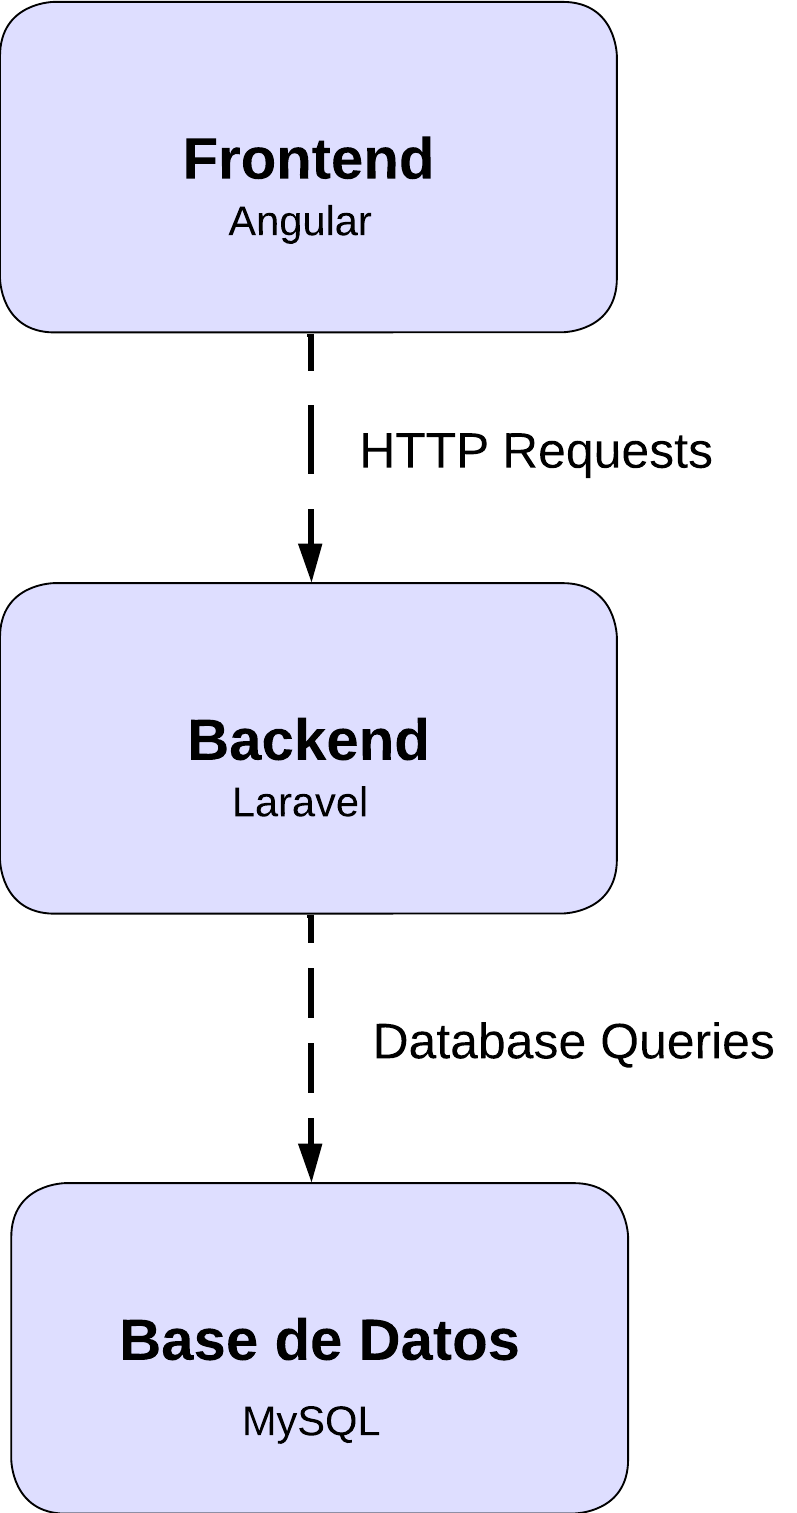
\includegraphics[scale=0.80]{./Images/diagramaTech.png}
\caption{Relación entre el Frontend (Angular), Backend (Laravel) y la Base de Datos (MySQL)}

\label{fig:fig1}

\end{center}
\end{figure}

El Frontend desarrollado en Angular envía peticiones HTTP al Backend, que utiliza el framework Laravel. Laravel gestiona las consultas de manera eficiente, permitiendo al backend comunicarse directamente con la base de datos MySQL, optimizando el acceso y la manipulación de los datos almacenados.

\section{Requisitos del proyecto}\label{sec:sec2.2}
En esta sección se detallan los requisitos que la aplicación debe cumplir para garantizar el éxito de su desarrollo:


\begin{itemize}
    \item La aplicación permitirá a los administradores gestionar el inventario de productos de pesca de forma integral, incluyendo la visualización en tiempo real del inventario y la capacidad de realizar actualizaciones en tiempo real.
    
    \item Se proporcionará una funcionalidad de ventas en línea que permita a los usuarios comprar productos de pesca directamente desde la aplicación web.
    
    \item Habrá un sistema de reservas de cebo integrado en la aplicación, que permitirá a los usuarios reservar cebo para su próxima salida de pesca.

    \item Los administradores podrán gestionar tanto los pedidos como las reservas de cebo. Cada vez que se realice un pedido o una reserva, se enviará un correo electrónico de confirmación tanto al cliente como al administrador.

    \item La aplicación contará con un sistema de autenticación de usuario para garantizar que solo los usuarios autorizados puedan acceder a determinadas funciones de la aplicación.

    \item El administrador podrá modificar la parte visual de la web, actualizando textos, imágenes y enlaces según sea necesario. Estos cambios permitirán reflejar nuevas ofertas, promociones o redirigir a los usuarios hacia secciones específicas del sitio web.

    \item La aplicación será diseñada con un enfoque en la seguridad y la usabilidad, asegurando que los datos de los usuarios estén protegidos y que la interfaz sea intuitiva y fácil de usar.
    
\end{itemize}